\documentclass{article}
\usepackage[utf8]{inputenc}
\usepackage[a4paper, total={6.5in, 10.3in}]{geometry}
\usepackage{merriweather}
\usepackage[hidelinks]{hyperref}
\usepackage{graphicx}
\usepackage{xcolor}
\usepackage{multirow}
\renewcommand{\baselinestretch}{1.22}
\usepackage{makecell}
\usepackage{minted}
\usepackage{subcaption}

% for markdown inline code effect
\definecolor{bgcolor}{HTML}{E0E0E0}
\let\oldtexttt\texttt
\renewcommand{\texttt}[1]{
  \colorbox{bgcolor}{\oldtexttt{#1}}
  }
 
% removing word break stuff
\tolerance=1
\emergencystretch=\maxdimen
\hyphenpenalty=10000
\hbadness=10000

\title{CS313: Lab Assignment 2}
\author{
  B Siddharth Prabhu\\
  \href{mailto:200010003@iitdh.ac.in}{\texttt{200010003@iitdh.ac.in}}
  }
\date{28 August 2022}

\begin{document}

\maketitle

\section{Answer to Question 1: Integrity Constraint Tabulation}
The below table contains all integrity constraints of the tables within the university schema at {\color{blue}\href{https://www.db-book.com/university-lab-dir/sqljs.html}{https://www.db-book.com/university-lab-dir/sqljs.html}} . Note that\texttt{VARCHAR(n)}refers to a variable-length {\color{red}\textit{\textbf{character}}} string that has a maximum length of n.\texttt{NUMERIC(n,m)}~refers to a {\color{red}\textit{\textbf{fixed point number}}} with user-specified precision of n digits, with m digits to the right of decimal point. 

\begin{table}[hbt]
    \centering
    \begin{tabular}{|p{2cm}|p{2.3cm}|p{2.5cm}|p{6cm}|p{1.5cm}|}
        \hline
         Table & Primary Key (PK) & Domain of PK & Foreign Key (Referencing Table) & Not Null 
         \\ %%%%%%%%%%%%%% classroom %%%%%%%%%%%%
         \hline \hline 
         \multirow{2}{*}{classroom} & building & VARCHAR(15) & \multirow{2}{*}{-}& \multirow{2}{*}{-}
         \\ \cline{2-3}
         & room\_number & VARCHAR(7) & & 
         \\ %%%%%%%%%%%%%% department %%%%%%%%%%%%
         \hline 
         department & dept\_name & VARCHAR(20) & - & - 
         \\ %%%%%%%%%%%%%% course %%%%%%%%%%%%
         \hline 
         course & course\_id & VARCHAR(8) & (dept\_name) references department & - 
         \\ %%%%%%%%%%%%%% section %%%%%%%%%%%%
         \hline
         \multirow{4}{*}{section} & course\_id & VARCHAR(8) & \multirow{4}{*}{\makecell[l]{(course\_id) references course, \\ \vspace{-3mm} \\ (building, room\_number) \\ \vspace{-3mm} references classroom}} & \multirow{4}{*}{-}
         \\ \cline{2-3}
         & sec\_id & VARCHAR(8) & & 
         \\ \cline{2-3}
         & semester & VARCHAR(6) & & 
         \\ \cline{2-3}
         & year & NUMERIC(4,0) & & 
         \\ %%%%%%%%%%%%%% instructor %%%%%%%%%%%%
         \hline 
         instructor & ID & VARCHAR(5) & (dept\_name) references department & name 
         \\ %%%%%%%%%%%%%% teaches %%%%%%%%%%%%
         \hline
         \multirow{5}{*}{teaches} & ID & VARCHAR(5) & \multirow{5}{*}{\makecell[l]{(course\_id, sec\_id, semester, year)\\ references section,\\ \vspace{-3mm} \\(ID) references instructor}} & \multirow{5}{*}{-}
         \\ \cline{2-3}
         & course\_id & VARCHAR(8) & & 
         \\ \cline{2-3}
         & sec\_id & VARCHAR(8) & & 
         \\ \cline{2-3}
         & semester & VARCHAR(6) & & 
         \\ \cline{2-3}
         & year & NUMERIC(4,0) & & 
         \\ %%%%%%%%%%%%%% student %%%%%%%%%%%%
         \hline
         student & ID & VARCHAR(5) & (dept\_name) references department & name 
         \\ %%%%%%%%%%%%%% takes %%%%%%%%%%%%
         \hline
         \multirow{5}{*}{takes} & ID & VARCHAR(5) & \multirow{5}{*}{\makecell[l]{(course\_id, sec\_id, semester, year)\\ references section,\\ \vspace{-3mm} \\(ID) references student}} & \multirow{5}{*}{-}
         \\ \cline{2-3}
         & course\_id & VARCHAR(8) & & 
         \\ \cline{2-3}
         & sec\_id & VARCHAR(8) & & 
         \\ \cline{2-3}
         & semester & VARCHAR(6) & & 
         \\ \cline{2-3}
         & year & NUMERIC(4,0) & & 
         \\ %%%%%%%%%%%%%% advisor %%%%%%%%%%%%
         \hline
         advisor & s\_ID & VARCHAR(5) & \makecell[l]{(i\_ID) references instructor (ID), \\ (s\_ID) references student (ID)} & -
         \\ %%%%%%%%%%%%%% time_slot %%%%%%%%%%%%
         \hline
         \multirow{4}{*}{time\_slot} & time\_slot\_id & VARCHAR(4) & \multirow{4}{*}{-} & \multirow{4}{*}{-}
         \\ \cline{2-3}
         & day & VARCHAR(1) & & 
         \\ \cline{2-3}
         & start\_hr & NUMERIC(2) & & 
         \\ \cline{2-3}
         & start\_min & NUMERIC(2) & & 
         \\ %%%%%%%%%%%%%% prereq %%%%%%%%%%%%
         \hline 
         \multirow{2}{*}{prereq} & course\_req & VARCHAR(8) & \multirow{2}{*}{\makecell{(course\_id) references course, \\ (prereq\_id) references course}}& \multirow{2}{*}{-}
         \\ \cline{2-3}
         & prereq\_id & VARCHAR(8) & & 
         \\ \hline
    \end{tabular}
    \caption{Integrity Constraints in university schema}
    \label{tab:my_label}
\end{table}

\section{Answers to Question 2: Getting all data of a particular student}
Let us consider all data of the student named `Shankar'. We can use natural joins to reduce column redundancy, OR we could use joins (manually) which may result in some redundancy. Either way, we get all the data we want corresponding to the student in question.

The queries used for retrieval of this info, accompanied by the respective output tables are as follows:
\\ \\
Using Natural Joins: \\
{
\emergencystretch=0
\fbox{ \begin{minipage}{45em}
\inputminted{mysql}{q2query1.sql}
\end{minipage}
}
}
\begin{figure}[hbt]
    \centering
    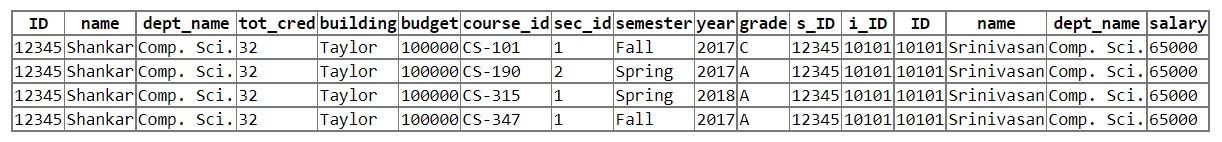
\includegraphics[scale=0.75]{q2query1op.jpg}
    \label{fig:my_label1}
\end{figure}

\\ \vspace{0.5cm}
{\noindent Using Joins:}\\(This is how the example given in the assignment worksheet appears to have been done)
\\
{
\emergencystretch=0
\fbox{ \begin{minipage}{45em}
\inputminted{mysql}{q2query2.sql}
\end{minipage}
}
}
\begin{figure}[hbt]
    \centering
    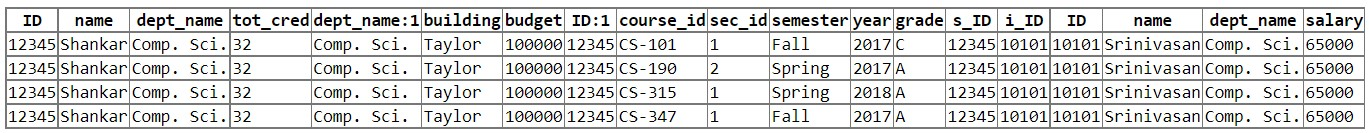
\includegraphics[scale=0.68]{q2query2op.jpg}
    \label{fig:my_label1}
\end{figure}
\\
\\

\noindent{What we can infer from the above tables is:}
A student named `Shankar' with ID = 12345 is in the Comp. Sci. department, and he has a total of 32 credits. His department is located in the `Taylor' building and has a budget of 100000. He has taken 4 courses, CS-101, CS-190, CS-315 and CS-347. The semester/year, sec\_id and grades for the same can be observed above. His advisor is an instructor named `Srinivasan' with ID = 10101 , who works in the Comp. Sci. department, and earns a salary of 65000.

\newpage
\section{Answers to Question 3: SQL SELECT and INSERT}
Here, we will explore the SQL commands SELECT and INSERT to construct and manipulate the tables of the the university schema. Firstly, we will insert records into the tables and observe the updations.
\\ \\ \\
{
\emergencystretch=0
\fbox{ \begin{minipage}{45em}
\inputminted{mysql}{q3insert.sql}
\end{minipage}
}
}
\newpage \noindent
{
\emergencystretch=0
\fbox{ \begin{minipage}{45em}
\inputminted{mysql}{q3insertmore.sql}
\end{minipage}
}
}
\\ \\ \\ Below are images of the insertions in `classroom' and `department':
\begin{figure}[hbt]
    \centering
    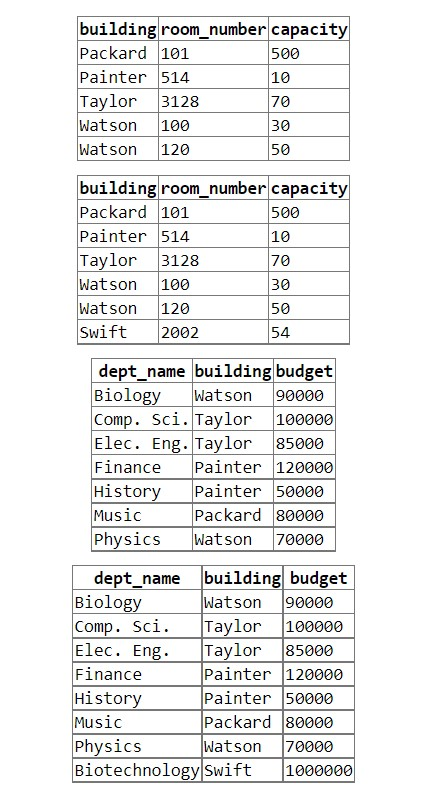
\includegraphics[scale=1.25]{pics/insert-pic1.jpg}
    \label{fig:ins1}
\end{figure} \newpage \noindent
Below are images of the insertions in `course':
\begin{figure}[!hbt]
    \centering
    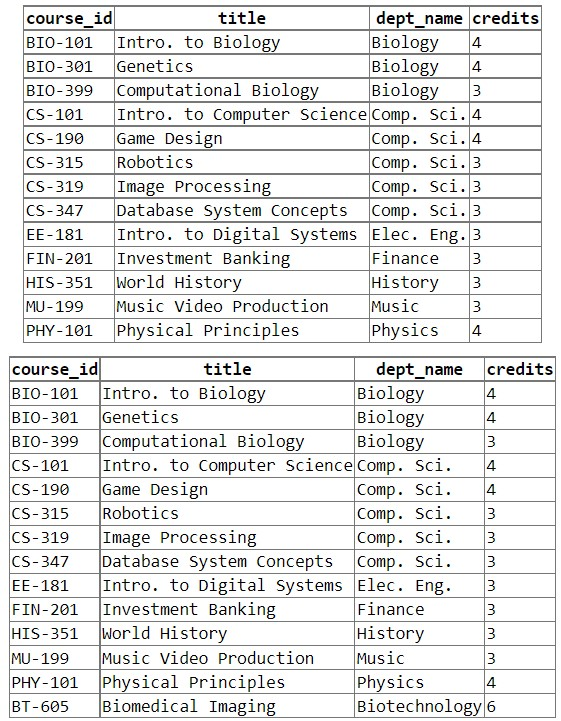
\includegraphics[scale=0.83]{pics/insert-pic2.jpg}
    \label{fig:ins2}
\end{figure} \\ \\ \\
Below are images of the insertions in `instructor':
\begin{figure}[!hbt]
    \centering
    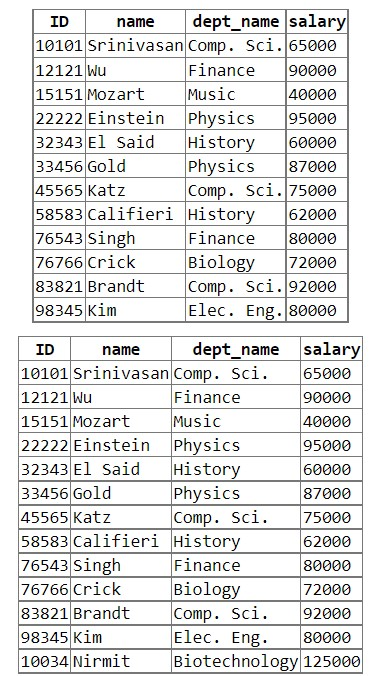
\includegraphics[scale=0.87]{pics/insert-pic3.jpg}
    \label{fig:ins3}
\end{figure} \newpage \noindent
Below are images of the insertions in `time\_slot':
\begin{figure}[!hbt]
    \centering
    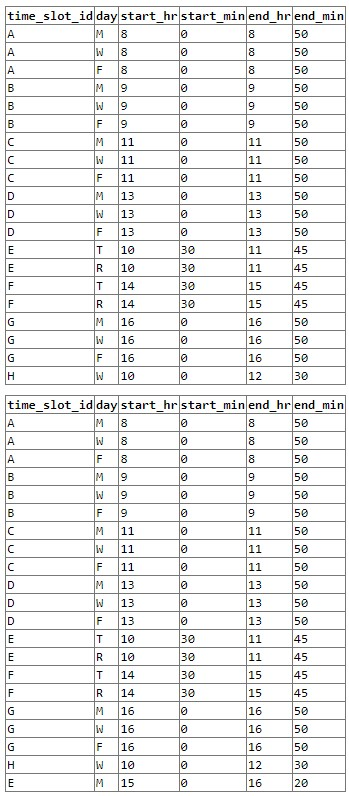
\includegraphics[scale=0.82]{pics/insert-pic4.jpg}
    \label{fig:ins4}
\end{figure} \\ \\ \\
Below are images of the insertions in `section':
\begin{figure}[!hbt]
    \centering
    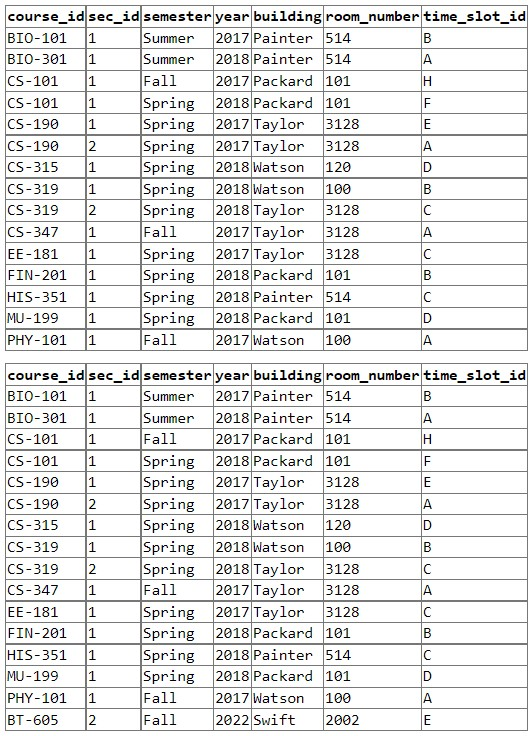
\includegraphics[scale=0.77]{pics/insert-pic5.jpg}
    \label{fig:ins5}
\end{figure} \newpage \noindent
Below are images of the insertions in `teaches':
\begin{figure}[!hbt]
    \centering
    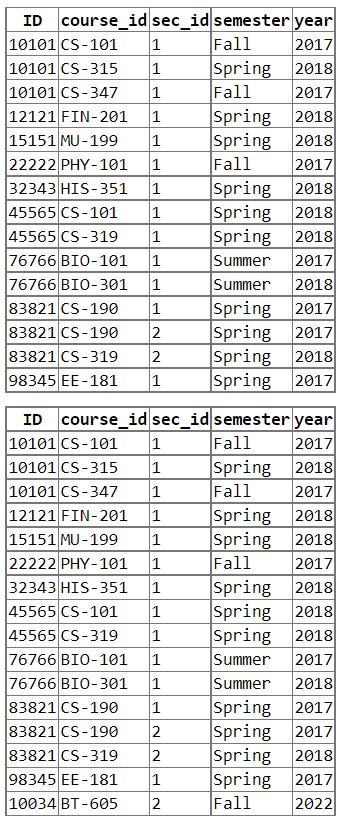
\includegraphics[scale=0.82]{pics/insert-pic6.jpg}
    \label{fig:ins6}
\end{figure} \\ \\
Below are images of the insertions in `student':
\begin{figure}[!hbt]
    \centering
    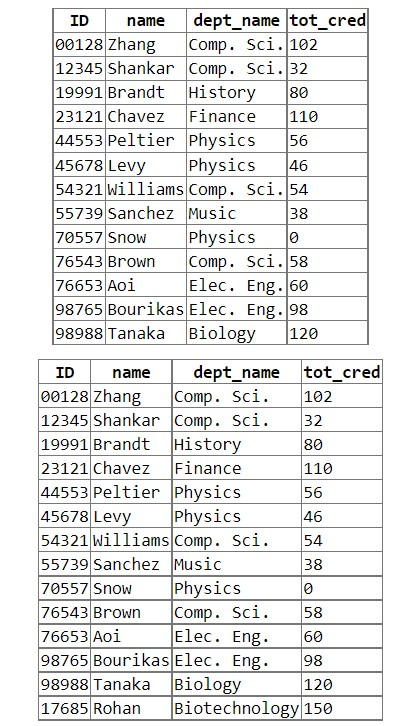
\includegraphics[scale=0.82]{pics/insert-pic7.jpg}
    \label{fig:ins7}
\end{figure} \newpage \noindent
Below are images of the insertions in `takes':
\begin{figure}[!hbt]
    \centering
    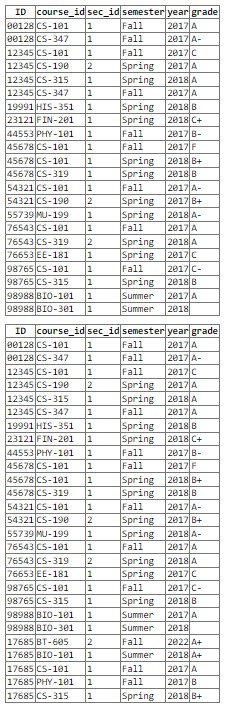
\includegraphics[scale=1.8]{pics/insert-pic8.jpg}
    \label{fig:ins8}
\end{figure}
\newpage \noindent
Below are images of the insertions in `advisor':
\begin{figure}[!hbt]
    \centering
    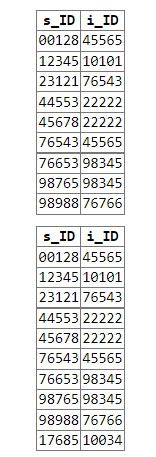
\includegraphics[scale=1.5]{pics/insert-pic9.jpg}
    \label{fig:ins9}
\end{figure} \\
Below are images of the insertions in `prereq':
\begin{figure}[!hbt]
    \centering
    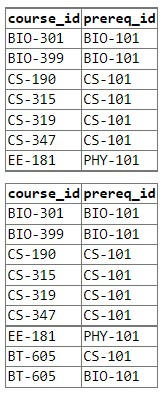
\includegraphics[scale=1.3]{pics/insert-pic10.jpg}
    \label{fig:ins10}
\end{figure} 

Now, let us explore more with the SELECT command, using different clauses, queries, and subqueries.
\newpage \noindent
{
\emergencystretch=0
\fbox{ \begin{minipage}{45em}
\inputminted[breaklines=true]{mysql}{q3select.sql}
\end{minipage}
}
}
\\ \\ \\ The output of the above queries is as follows:
\begin{figure}[!hbt]
    \centering
    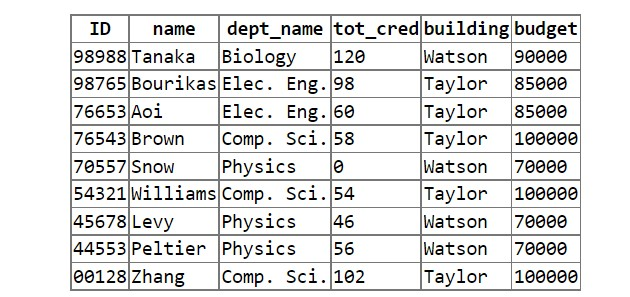
\includegraphics[scale=1.2]{pics/select-pic1.jpg}
    \label{fig:sel1}
\end{figure} \newpage \noindent
\begin{figure}[!hbt]
    \centering
    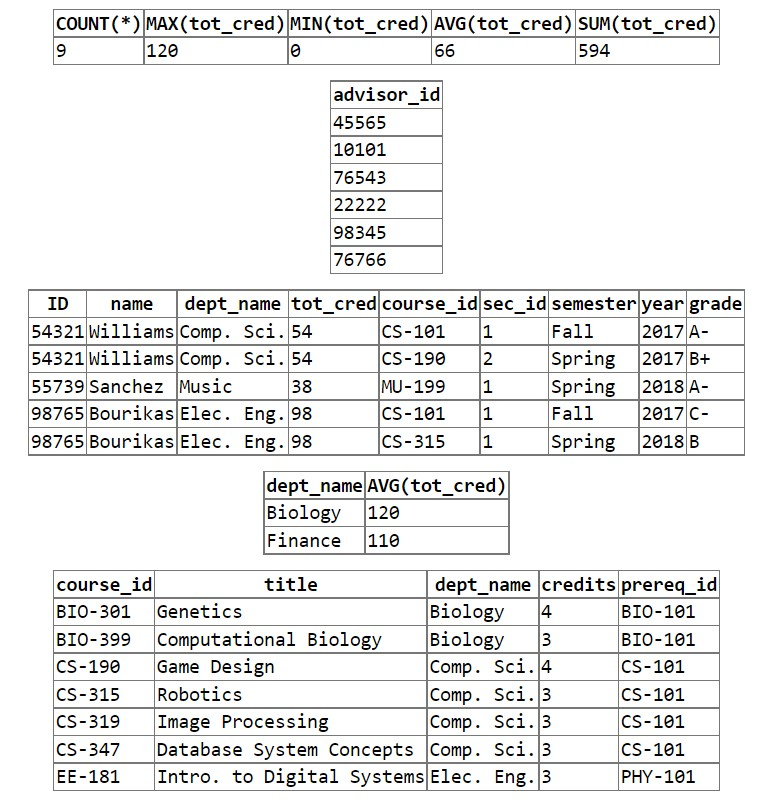
\includegraphics[scale=1.2]{pics/select-pic2.jpg}
    \label{fig:sel1}
\end{figure}

\section{Answers to Question 4: More Queries!}
\subsection{(a) Which students study in x department and y building?}
Let x be `Physics' department and y be `Watson' building. Then, the code would entail the following query: \\
{
\emergencystretch=0
\fbox{ \begin{minipage}{45em}
\inputminted{mysql}{q4query1.sql}
\end{minipage}
}
} \\ \\
Note that we can't use the `building' given in the `department' table, since we need the \underline{\textbf{building in which the student attends classes}}, and not the building corresponding to the student's dept\_name.  The output of the above is in the following table (next page):
\newpage \noindent
\begin{figure}[!hbt]
    \centering
    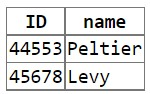
\includegraphics{pics/q4-pic1.jpg}
    \label{fig:q4p1}
\end{figure}
\subsection{(b) Which students have A grade as well as C grade?}
The code and output image for this are as follows: \\
{
\emergencystretch=0
\fbox{ \begin{minipage}{45em}
\inputminted{mysql}{q4query2.sql}
\end{minipage}
}
} \\
\begin{figure}[!hbt]
    \centering
    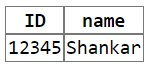
\includegraphics{pics/q4-pic2.jpg}
    \label{fig:q4p2}
\end{figure}
\subsection{(c) Where do classes happen on Wednesday?}
The code and output image for this are as follows:\\
{
\emergencystretch=0
\fbox{ \begin{minipage}{45em}
\inputminted{mysql}{q4query3.sql}
\end{minipage}
}
} \\
\begin{figure}[!hbt]
    \centering
    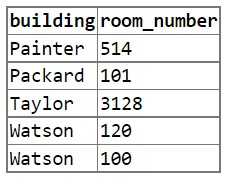
\includegraphics{pics/q4-pic3.jpg}
    \label{fig:q4p2}
\end{figure}

\newpage
\section{For reference: Given university Schema}
\begin{figure}[!hbt]
    \centering
    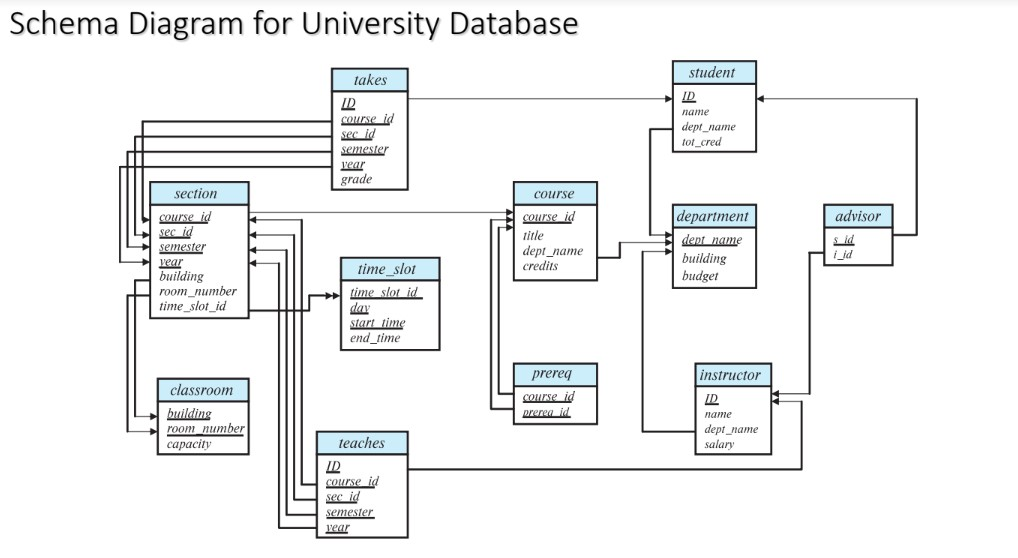
\includegraphics{schema.jpg}
    \caption{Caption}
    \label{fig:my_label}
\end{figure}

\end{document}
